%%%%%%%%%%%%%%%%%%%%%%%%%%%%%%%%%%%%%%%%%
% Simple Sectioned Essay Template
% LaTeX Template
%
% This template has been downloaded from:
% http://www.latextemplates.com
%
% Note:
% The \lipsum[#] commands throughout this template generate dummy text
% to fill the template out. These commands should all be removed when 
% writing essay content.
%
%%%%%%%%%%%%%%%%%%%%%%%%%%%%%%%%%%%%%%%%%

%----------------------------------------------------------------------------------------
%	PACKAGES AND OTHER DOCUMENT CONFIGURATIONS
%----------------------------------------------------------------------------------------

\documentclass[12pt]{article} % Default font size is 12pt, it can be changed here

\usepackage{geometry} % Required to change the page size to A4
\geometry{a4paper} % Set the page size to be A4 as opposed to the default US Letter

\usepackage{graphicx} % Required for including pictures

\usepackage{float} % Allows putting an [H] in \begin{figure} to specify the exact location of the figure
\usepackage{wrapfig} % Allows in-line images such as the example fish picture

\usepackage{lipsum} % Used for inserting dummy 'Lorem ipsum' text into the template

\linespread{1.2} % Line spacing

%\setlength\parindent{0pt} % Uncomment to remove all indentation from paragraphs

\graphicspath{{Pictures/}} % Specifies the directory where pictures are stored

% Custom
\usepackage{blindtext} %  for quote
\usepackage{textcomp}

\begin{document}

%----------------------------------------------------------------------------------------
%	TITLE PAGE
%----------------------------------------------------------------------------------------

\begin{titlepage}

\newcommand{\HRule}{\rule{\linewidth}{0.5mm}} % Defines a new command for the horizontal lines, change thickness here

\center % Center everything on the page

\textsc{\LARGE Galway Mayo Institute of Technology}\\[1.5cm] % Name of your university/college
\textsc{\Large Software Development}\\[0.5cm] % Major heading such as course name
\textsc{\large Literature Review}\\[0.5cm] % Minor heading such as course title

\HRule \\[0.4cm]
{ \LARGE \bfseries The advantages of using JavaScript for full stack development with an emphasis on Node.js}\\[0.4cm] % Title of your document
\HRule \\[1.5cm]

\begin{minipage}{0.4\textwidth}
\begin{flushleft} \large
\emph{Author:}\\
Ronan \textsc{Connolly} % Your name
\end{flushleft}
\end{minipage}
~
\begin{minipage}{0.4\textwidth}
\begin{flushright} \large
\emph{Supervisor:} \\
Dr. Sean \textsc{Duignan} % Supervisor's Name
\end{flushright}
\end{minipage}\\[4cm]

{\large \today}\\[3cm] % Date, change the \today to a set date if you want to be precise

%\includegraphics{Logo}\\[1cm] % Include a department/university logo - this will require the graphicx package

\vfill % Fill the rest of the page with whitespace

\end{titlepage}

%----------------------------------------------------------------------------------------
%	TABLE OF CONTENTS
%----------------------------------------------------------------------------------------

\tableofcontents % Include a table of contents

\newpage % Begins the essay on a new page instead of on the same page as the table of contents 

%----------------------------------------------------------------------------------------
%	INTRODUCTION
%----------------------------------------------------------------------------------------

\section{Introduction} % Major section
% Basic intro to JS
Currently JavaScript is the only language that we can use to develop both web based applications in both the client and the server side \cite{5}.

Using JavaScript throughout both the client and server allows developers to advance their knowledge to a deeper level than time would usually allow \cite{1}.

By using just JavaScript on the server side and for cloud side applications, we can promote software re-usability and bring some order to the chaos that is heterogeneity \cite{2}.

The quite recent introduction of Google's V8 Engine, CSS3, HTML5 and the lower hosting costs has altered the web a lot. Since these changes there has been an explosion in web-based applications being developed by even the most novice developer \cite{3}.

There are many server-side frameworks available such as Java's Spring, Python's Django, PHP's CodeIgnitor/Zend, Ruby's Rails and JavaScript's Node.js. Node.js (from now on to be referred to simply as Node) is special in the way that it solves well-known challenges in teaching web development. Node allows for the consolidation of language throughout the language stack. The platform supports a smooth learning curve, allowing developers to build their knowledge gradually through the use of modular, open source components. As web technologies progress, these new frameworks offer increased utility and distributed connectivity \cite{1}.

% talk about what we're covering in this paper and where JS is going.
This short paper endeavors to clarify some of the thinking behind using JavaScript for full-stack development and beyond. Full-stack meaning where JavaScript is used on both the client and the server. Beyond meaning using JavaScript for many other uses, utilising NoSQL technologies such as CouchDB and MongoDB, using packages like Fuzzy.io for Artificial Intelligence, or Johnny Five for the Internet of Things. There is such a vibrant community of JavaScript developers out there pushing the threshold of what JavaScript is and can do. 
With the soon arrival of ECMA Script 2015 (known to many as JavaScript6 or ECMAScript 6), things are only going to improve for the JavaScript community. Many ideas and Object Oriented Fundamentals like lexical scope binding, classes and sets/maps are included in the update.
I will describe the asynchronous nature of Google's V8 nature, how node has taken advantage and why it's pushing JavaScript forward as a winner for full-stack development. I will also touch on a few problems people may encounter on their endeavors with JavaScript and Node.

%----------------------------------------------------------------------------------------
%	Current Issues with Heterogeneity
%----------------------------------------------------------------------------------------

\section{Heterogeneity} % Sub-section
Stepp \cite{9} has published informal survey results which indicate HTML/CSS and JavaScript are covered in virtually every course covering client-side development - their dominance on the client-side leaves little choice in adoption. There is little consensus on the server however, with PHP, Java/JSP, Ruby on Rails, ASP.NET, and Python being common choices among educators \cite{1}.

Having JavaScript already being the number one choice for client side development, NoSQL technologies primarily being used with JavaScript and with Node rising in popularity, it makes sense to consider using JavaScript for full-stack development.

It can take quite a bit of time constantly switching between different frameworks and languages. If you are using just one language and a handful of similar frameworks (more then likely in the same community of developers), you will be able to gain a deeper understanding and come up with more interesting and vibrant solutions.

We should remove the trivial and mundane task of doing a context switch from one language to another. Edsgar Dijkstra believed that programming wasn't about writing code but about coming up with new solutions to problems:
``In order to compose, you have to write scores, but to be a composer is not to write scores; to be a composer is to conceive music ''\cite{10}.
It was a different time when he said this, C was the higher language and he was referencing machine code as being analogous to writing scores but the point still prevails, the need to remove trivial mundane tasks is of utmost importance, this leads to smarter solutions for more efficient code.

%----------------------------------------------------------------------------------------
%	How Javascript can solve this problem
%----------------------------------------------------------------------------------------

\section{JavaScript} % Sub-section

The original and dominant use of JavaScript remains in web applications run in a web browser. Here, events are emitted in response to user actions like mouse clicks or keyboard presses, and internal browser events like the completion of a network request. Events are propagated along the structure of the HTML document, using the event capturing and bubbling strategies. Listeners are attached to HTML elements and can cancel (stop the propagation) of events programatically.

With the event-driven JavaScript interpreter like Google's V8 VM that Node is based on, applications register an interest in certain events, like when data is ready to be read on a certain socket.
Asynchronous I/O is important for event-driven programming because it prevents the application from getting blocked while waiting for an I/O operation.
Event-driven programming can be problematic just like multi-threaded programs. One of these problems is that not all inter-process communication can be tied into the event notification facilities. The sheer complexity of writing asynchronously in some languages like C can be incredibly perplexing. As Tilkov et al. states ``Many such applications end up being little more than impenetrable, un-maintainable tangles of spaghetti code and global variables.'' \cite{4}.

\begin{quote}
% \blindtext
\itshape By the way, on the matter of hype: People have always been quick to announce ``the next software development revolution,'' usually about their own brand-new technology. Don't believe it. New technologies are often genuinely interesting and sometimes beneficial, but the biggest revolutions in the way we write software generally come from technologies that have already been around for some years and have already experienced gradual growth before they transition to explosive growth. This is necessary: You can only base a software development revolution on a technology that's mature enough to build on (including having solid vendor and tool support), and it generally takes any new software technology at least seven years before it's solid enough to be broadly usable without performance cliffs and other gotchas. As a result, true software development revolutions like OOP happen around technologies that have already been undergoing refinement for years, often decades. Even in Hollywood, most genuine ``overnight successes'' have really been performing for many years before their big break.
\hfill Herb Sutter \cite{11}
% \par
% \begingroup
% \leftskip4em
% \rightskip\leftskip
% \blindtext
% \par
% \endgroup
% \blindtext
\end{quote}

Whatever you think about JavaScript as a programming language, there is little doubt that it has come about as being the dominant language of choice when doing any web development work or any HTML based application such as Electron (desktop apps) or Ionic (mobile apps).

Server-side JavaScript is a logical next step, enabling the use of a single programming language for all aspects of a distributed web-based application.
Server-side JavaScript isn't yet a mainstream approach as it's only recently gotten huge exposure due to Node.

\subsection{ES2015} % Sub-section
ES2015 is the newest update to arrive for JavaScript, it arrived in June 2015. It is the biggest update since the introduction of JavaScript by Netscape (Brendan Eich) in 1995.
It was originally planned to be called ECMAScript6 but they revised the naming convention and changed it to ES2015, and from now on there will be a release every year following the new naming convention.
ECMAScript6: is the next version of JavaScript standard, it brings a variety of features found in other languages such as Java and C for creating high-performance applications to JavaScript \cite{2}. Two really important features are Promises and Typed Arrays.

Asynchronous programming introduces a simplified way to handle operations, as opposed to conventional callback-based approaches. ``Promises'' bring a structured flow to applications by chaining events so that the order of events is guaranteed. It does so with the aid of a newly introduced method called ``then'', which takes two parameters - success and error callbacks \cite{2}.

Promises have being available through external libraries such as ``Q'' and ``Async'' but now they will be introduced fully into the language.

With the upcoming introduction of ``Promise as a language feature'', we expect an increase in interest, and believe that many developers will shift to this better practice of using promises rather then callbacks as stated by E. Brodu et al. in \cite{7}.

Promises were introduced to solve the problem of the constant use of callbacks that leads to intricate imbrications of function calls and callbacks, commonly known as ``callback hell'' or the ``pyramid of doom''. Basically where there can be a mess of nested callbacks in the code.

%----------------------------------------------------------------------------------------
%	Why Node.js is great for the server side
%----------------------------------------------------------------------------------------

\section{Node.js} % Sub-sub-section

Node is a hugely successful platform that combines the popular JavaScript language with an efficient runtime tailored for a cloud-based architecture. 
JavaScript has many advantages for web development. It is the de facto dominant language for client-side applications and it offers the flexibility of dynamic languages. In particular it allows the easy combination or mash-up of content and libraries from varying third parties\cite{12}. This works perfectly with Node as we can easily plug in different modules with a simple ``npm install \textlangle{}package\textrangle{}'' from the command line.
It has never been so easy to go from design and development to testing and production.

Currently, a server environment for running a Node application can be easily created and/or accessed on a cloud server, and thus, a run-time environment is obtained without the user/developer explicitly having to install any software. This may result in a change in the business model of software applications \cite{13}.

\begin{figure}[H] % Example image
\center{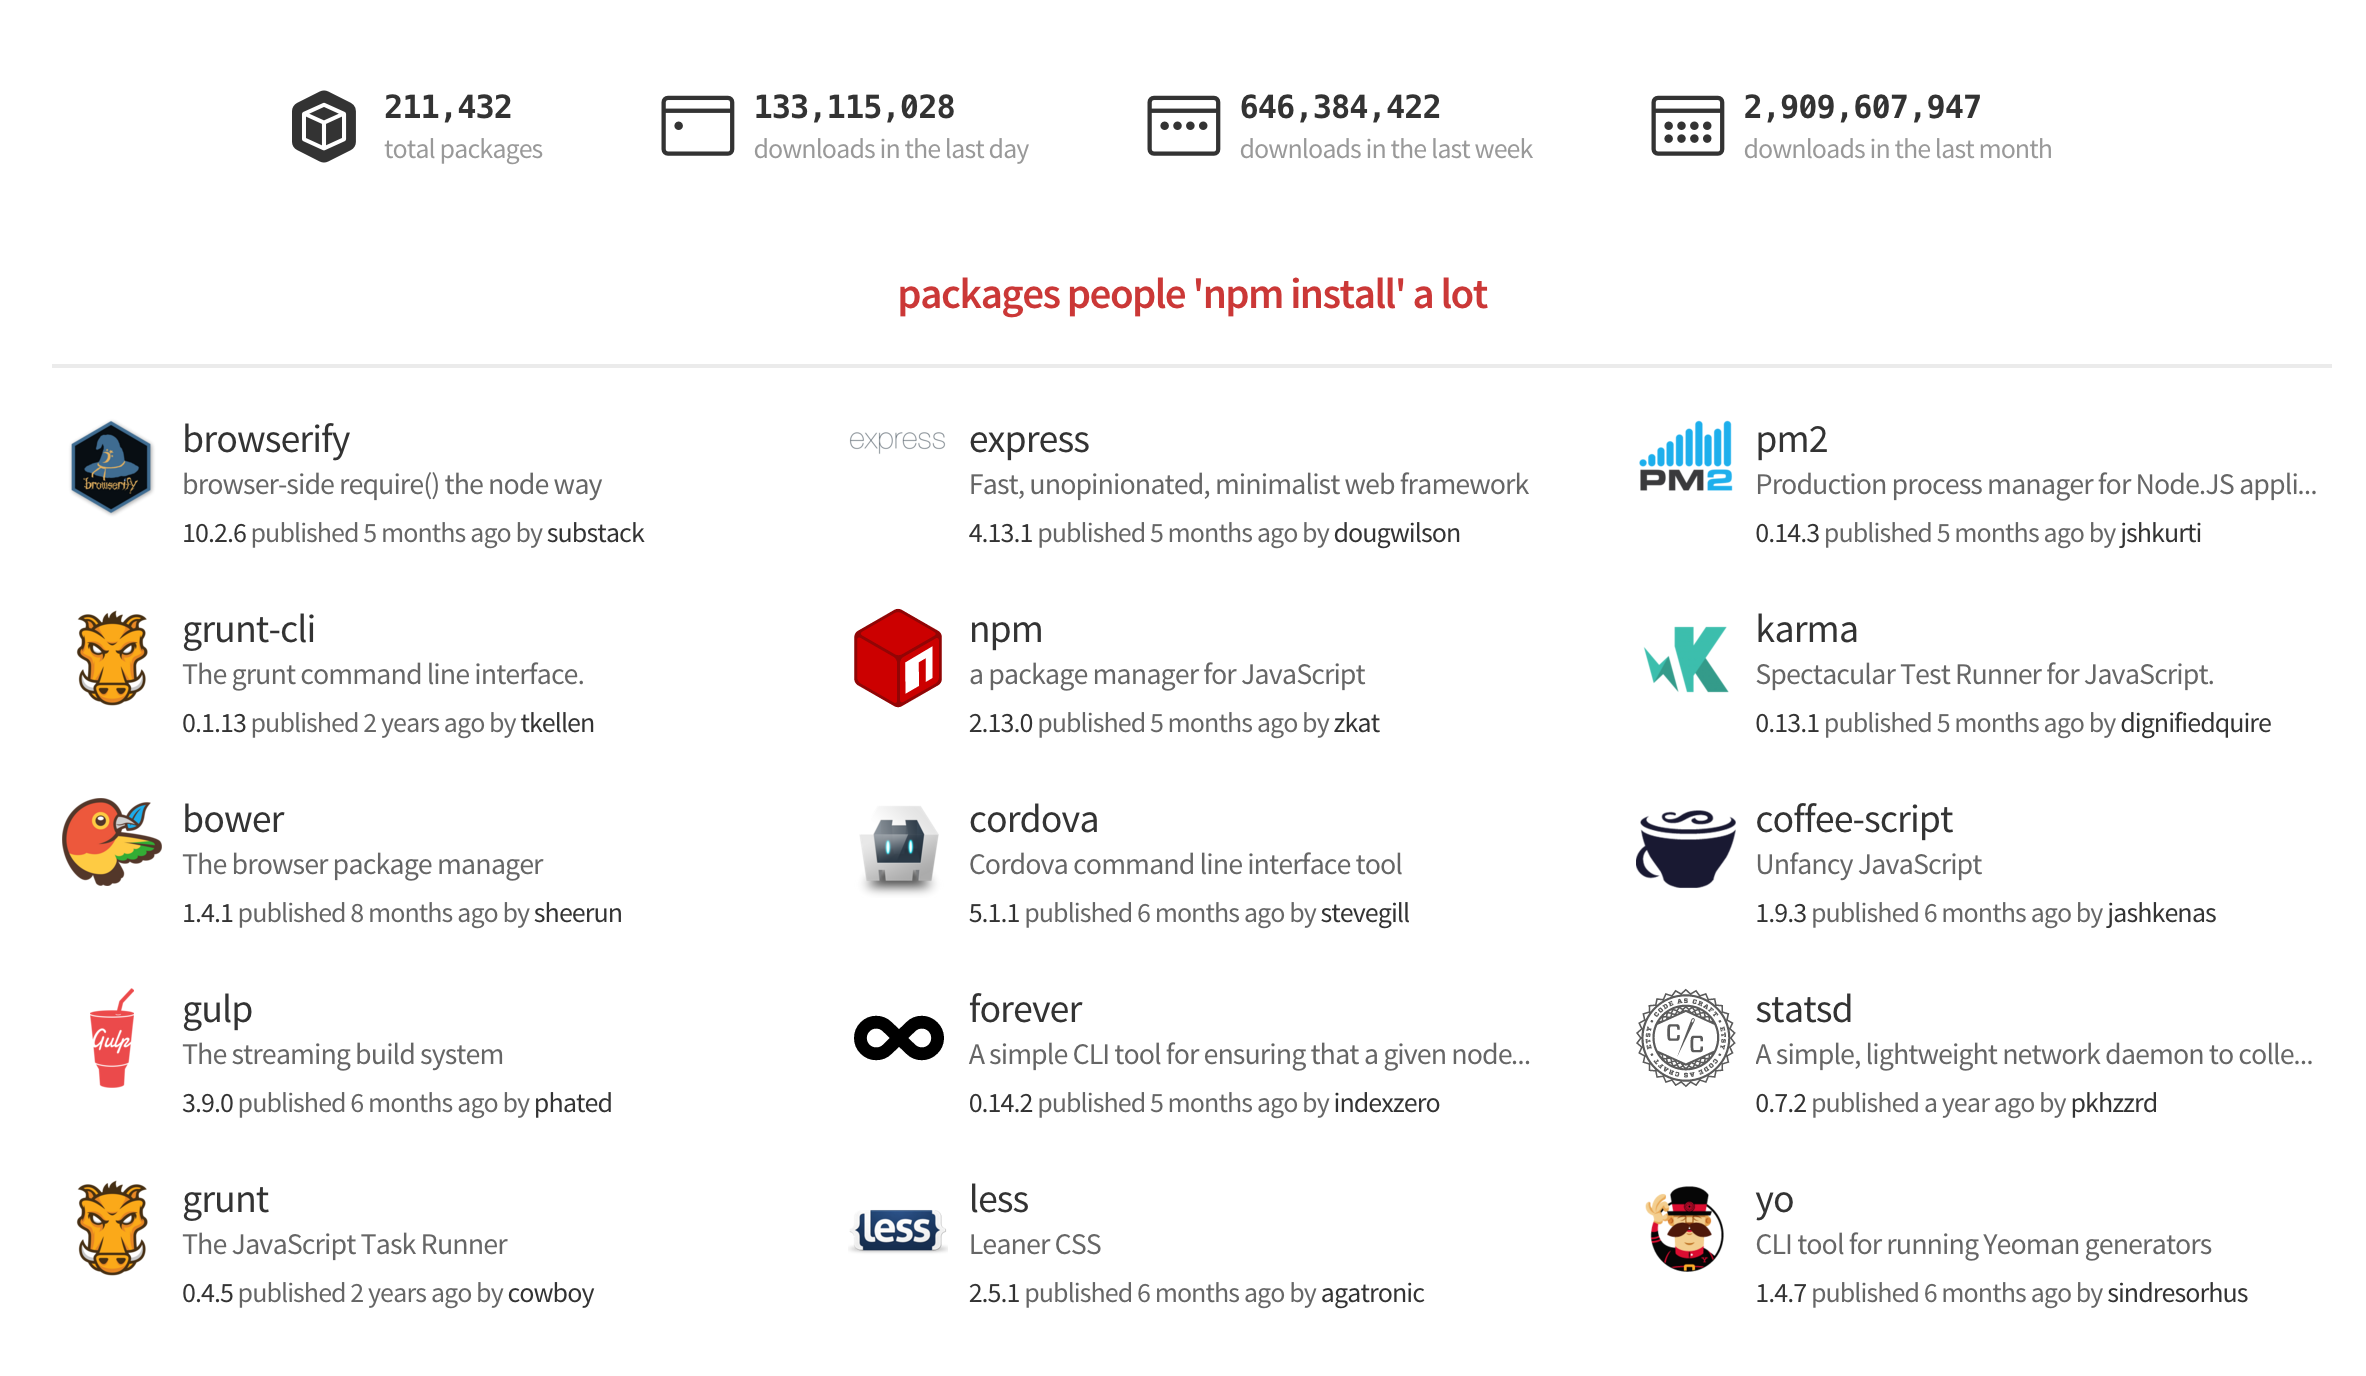
\includegraphics[width=1.0\linewidth]{npm}}
\caption{NPM Homepage}
\label{fig:speciation}
\end{figure}
As eveidence to the popularity of Node, the NPM package repository has recently surpassed Maven Central and Ruby Gems with more than 211,377 available packages and over 250 packages added every day \cite{8}. 
Just last month as you can see from figure 1 above, there were 2,909,607,947 downloads from the NPM package repository.

Some of the most popular NPM packages are ``jade'', ``grunt'', ``mongoose'', ``socket.io'', ``express'', ``browserify'' and ``gulp''. These packages contain many packages themselves, creating a kind of tree like structure. Packages within packages, etc. Many of the mentioned packages contain more then 200 libraries each. ``express'' includes 138 packages \cite{12}.

Among the various server-side frameworks, Node has emerged as one of the most popular. Its strengths are the use of JavaScript, an efficient run-time tailored for cloud-based event parallelism, and thousands of third-party libraries \cite{12}.

\subsection{Interpreter and Threads}
First what is the JavaScript interpreter and who built it?
% JS Interpreter, Google V8, asynchronous
Node is a JavaScript interpreter based on Google's V8 virtual machine. It's designed to use 
asynchronous input/output by default, including an event model which makes event-driven programming really easy. Since it is basically a JavaScript interpreter, sequential and synchronous programs are possible and, because of the speed of the underlying JavaScript virtual machine, it has high performance, but the best way of utilizing it is by taking advantage of the asynchronous I/O features that make it different from other JavaScript interpreters such as Spider-monkey or Rhino and, in fact, closer to the event-driven programming that is usual in browsers \cite{6}.

% node single threaded
You should try to think of the Node server process as a single-threaded daemon that contains the JavaScript engine to support customization. This is quite different from most eventing systems for other programming languages, which come in the form of libraries. The eventing model in Node is supported at the language level. JavaScript is great for this approach because it supports event callbacks.
For example, when a browser completely loads a document, a user clicks a button, or an Ajax request is fulfilled, an event triggers a callback. JavaScript's functional nature makes it extremely easy to make anonymous function objects that you can register as event handlers \cite{4}.

% Used for multi-threaded as using JS event loop
Although many developers have successfully used multi-threading in production applications, most of them will agree that multi-threaded programming is very difficult. It has many problems that can be difficult to find and fix, such as deadlock and failure to protect resources shared among threads. Developers also lose some degree of control when drawing on multi-threading because the OS typically decides which thread executes and for how long. Event-driven programming offers a more efficient, scalable alternative that provides developers much more control over switching between application activities \cite{4}.

\subsection{Why Node?}
% node summary
The I/O approach Node takes is strict. Its Asyncronous interactions aren't the exception, they're the rule. All of Nodes I/O operations are handled by higher-order functions (functions taking functions as a parameter), that state what happens when there is something to do \cite{4}.
JavaScript is a functional language (but not purely functional) and as such, supports higher-order functions. When writing Node programs you will see functions everywhere. The main flow of the program is 

The programs main flow is set by the functions that are explicitly called. These functions never block anything I/O related, but rather register appropriate handler callbacks. If you've seen a similar concept in other eventing libraries you may be wondering where the event loop hides?

\begin{wrapfigure}{l}{0.70\textwidth} % Inline image example
  \begin{center}
    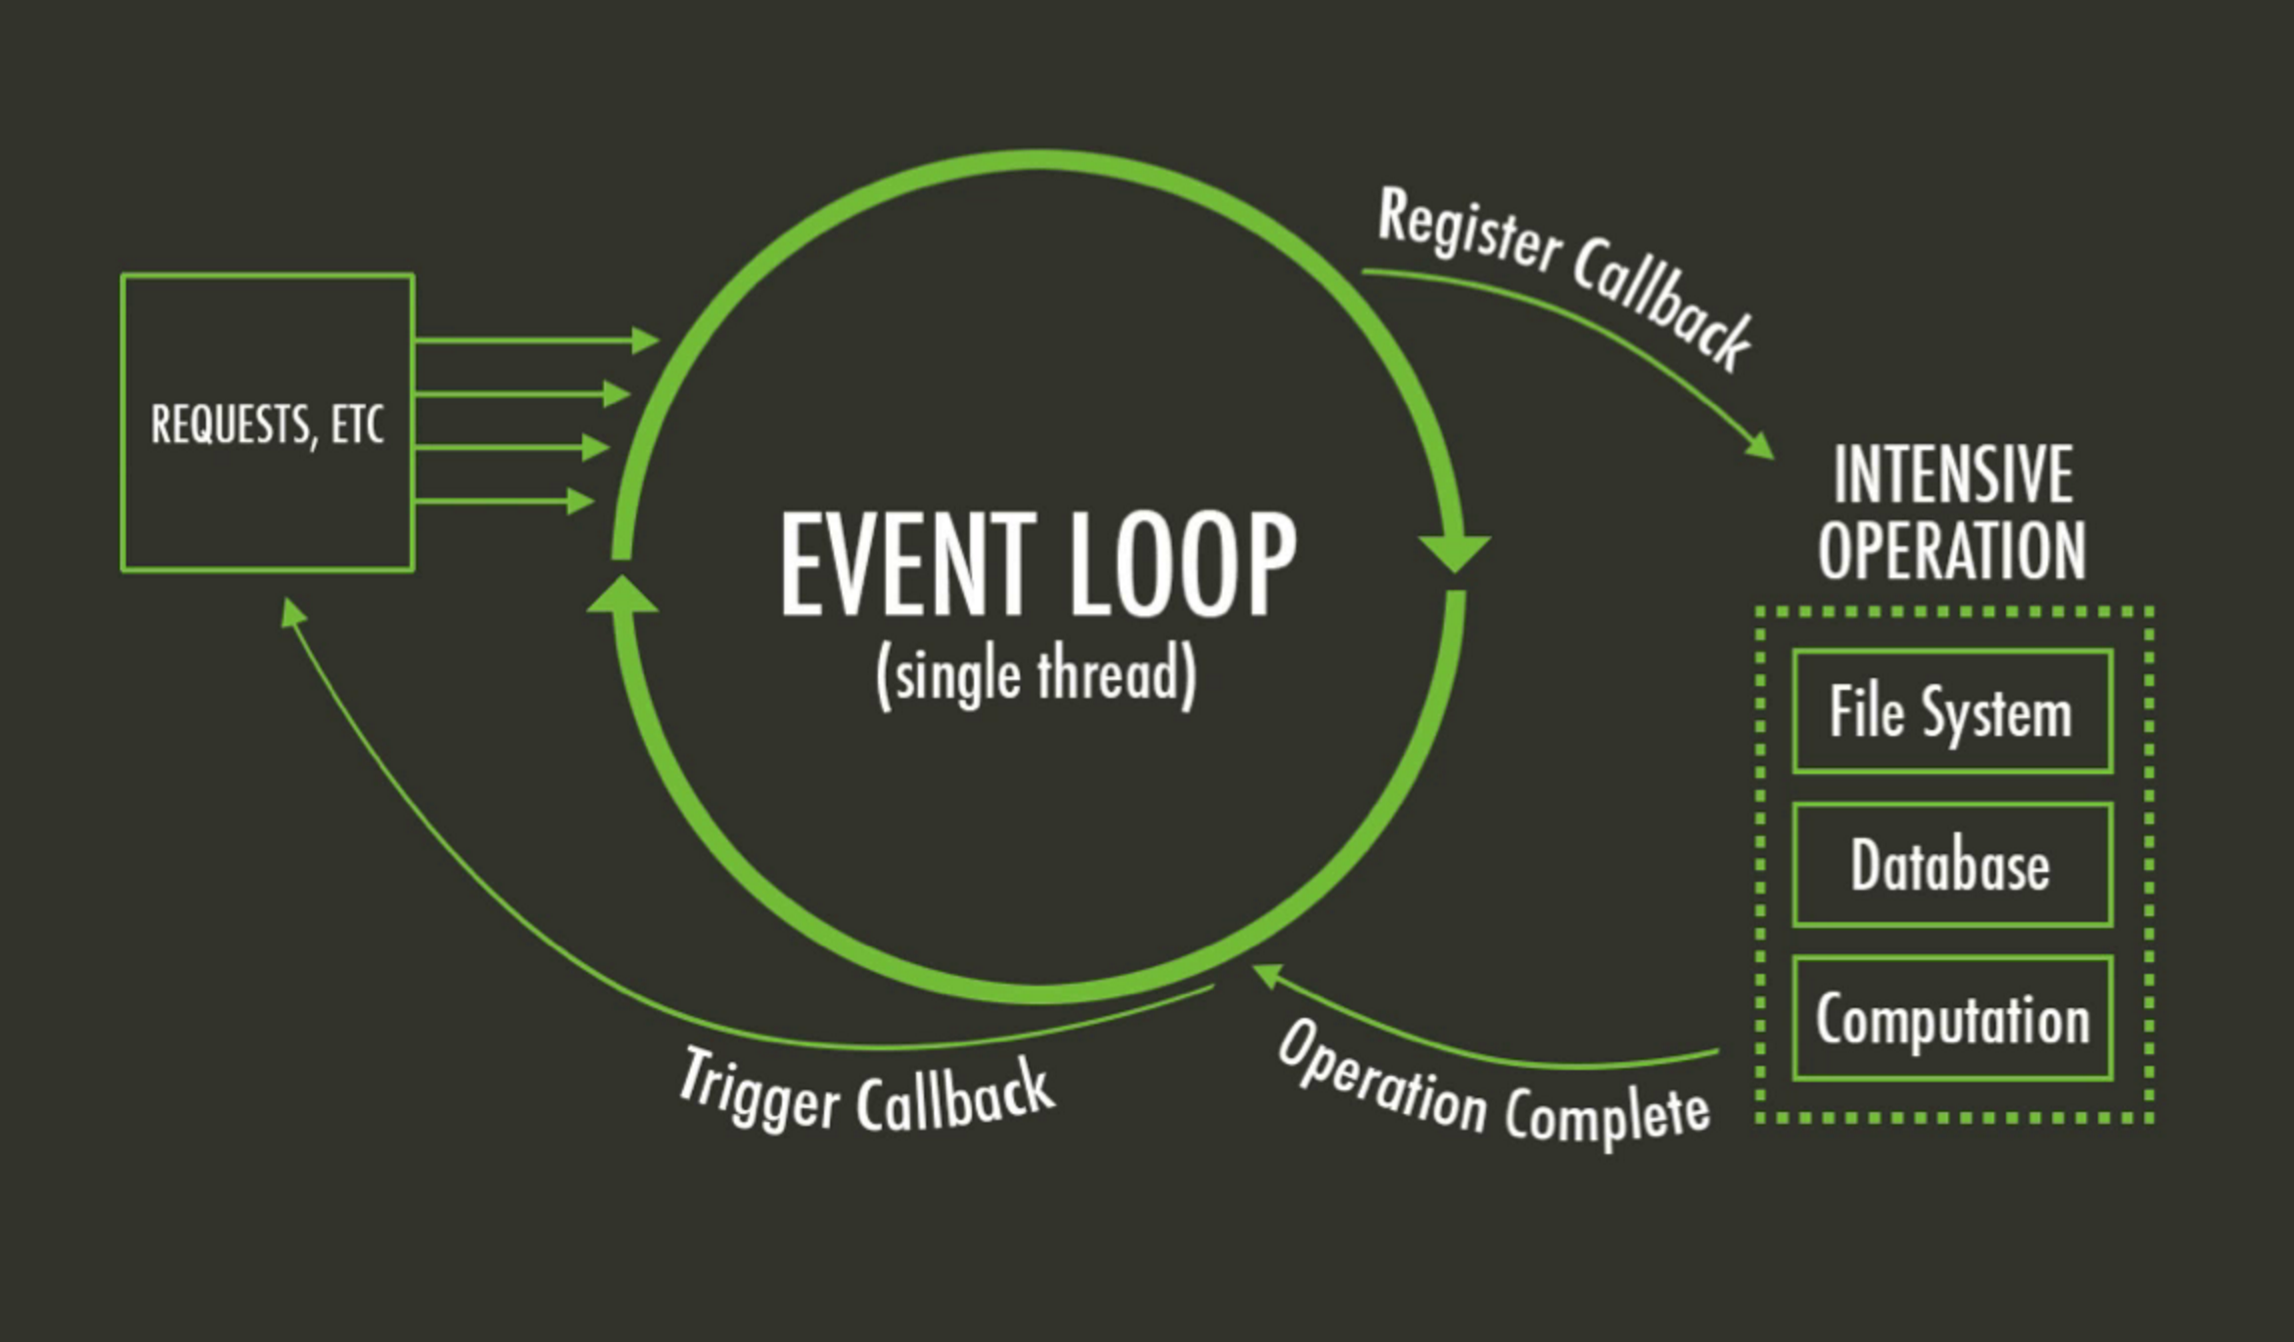
\includegraphics[width=0.68\textwidth]{loop}
  \end{center}
  \caption{Node Event Loop}
\end{wrapfigure}

The event loop idea is so important in Node's behavior  that it hsa hidden the implemenation of it.
The main purpose of the program is to simply set up appropriate handlers \cite{4}.
Lots of registration calls happen in the loop, no actual I/O happens.
By having asyncronous I/O as the default forces developers to use the asyncronous model from the beginning, this is one of the main differences between other Node and asyncronous I/O in other programming environments, where this would be thought of as too complex or advanced.

Google's V8 engine (created in C++) on which Node is based uses JIT (just in time) compilation to achieve near-native performance, hugely outperforming traditional interpreter-based approaches\cite{1}.

Importantly, the V8 engine (created in C++) on which Node is based uses JIT (just in time) compilation to achieve near-native performance, vastly outperforming traditional interpreter-based approaches\cite{1}.

In most web development projects JavaScript knowledge is a prerequisite  and the option of usin just one programming language for everything becomes quite tempting. Node's architecture makes it very easy to yse a highly expressive, functional language for server-side programming, without any sacrifice on performance \cite{4}.

Node deeply embraces the Unix style of programming, encouraging small, interchangable modules.
When you look closely at an many Node programs, you will see similar concepts to those seen in Unix, like for instance piping input and output streams in sockets, files and stdin \cite{1}. 

What's unique about Node is it's ability to provide a high level of language consistency using JavaScript across all facets of the stack (back-end, front-end, database, etc). It provides a distinct mix of high-level abstraction and at the same time an exposure to low level detail \cite{1}.

% \begin{figure}[H] % Example image
% \center{\includegraphics[width=0.5\linewidth]{placeholder}}
% \caption{Example image.}
% \label{fig:speciation}
% \end{figure}

%------------------------------------------------
%	Issues with node
%------------------------------------------------

\section{Is JavaScript always the best?}
I have laid out arguments about the speed of JavaScript through the use of Google's V8 engine and in such the speed of programs using the Node platform.
The V8 runtime environment on which Node is based (and javascript applications run in Google's Chrome browser) is extremely fast and achieves near native speed due to JIT (just in time) compilation. JIT works by compiling certain sections of code based on heuristics laid out by the runtime environment. These heuristics could be based on code segments that are more likely to be used. When code is compiled is is kept in memory in a cache (so as not to have to compile it multiple times). This gives applications near native performance, everybody can agree that Oracles JVM JIT compilation gives excellent speeds, but that is compiling ``bytecode'', in V8 we are compiling source code. Runtime environments utilising JIT compilation tend to have a ``warming up'' phase where the program may lag abit, then once a sufficient amount of code is compiled the near native performance kicks in.

There is a spectrum between native and interpreted languages. Native sits on one side and interpreted on the other.
There will always be a space for native code (developed with the likes of C++) where performance is key like for things such as gaming and stock trading, but for portability, scalability, testing and ease of use JavaScript is on top, although you do take a performance hit due to the interpretation that takes place.
Then you have intermediately compiled languages like Java that sit in the middle of the spectrum, which compiles to bytecode, is portable (to any machine that has a JVM set up) and achieves near native performance (through JIT compilation). 

Since all you need to run JavaScript is a browser (which every computer has, compared to Java where you have to install the JVM) and with the recent introduction of object oriented concepts and new collection types in ES2015 JavaScript is started to get closer performance to Java.

This is a space to be watched.

\section{JavaScript Beyond} % Sub-sub-section
We now understand the power of JavaScript on the server and client side but there are many other areas that developers can transfer their JavaScript knowledge to.

With the introduction of WebGL (an implementation of OpenGL in JavaScript), JavaScript can be used to create amazing simulations and 3D games within a web browser.

NoSQL (not only SQL) technologies like CouchDB, MongoDB and Neo4J are becoming more and more popular. MongoDB stores it's data in JSON format and uses a JavaScript syntax for all of it's administration \& querying facilities; and so do many other frameworks \cite{1}.

The Cordova project has brought the power of low level phone components (called hooks) into the hands of JavaScript developers, hooks allow developers to use things like GPS, Bluetooth, Gyroscope and other hardware components in a webview within an app. This means you can create an entire mobile application using JavaScript. Adobes PhoneGap has built off of Cordova, and the very successful Ionic is built on top of Cordova.
The Ionic team have created an amazing framework for building modern mobile applications with ease in JavaScript, mobile apps that can truly stand up against native apps.

Achieving competency in JavaScript allows a developer to quickly become productive with these growing technologies.


%----------------------------------------------------------------------------------------
%	MAJOR SECTION 1
%----------------------------------------------------------------------------------------

% \section{Content Section} % Major section

% \lipsum[5] % Dummy text

%------------------------------------------------

% \subsection{Subsection 1} % Sub-section

% \subsubsection{Subsubsection 1} % Sub-sub-section

% \lipsum[6] % Dummy text

%------------------------------------------------

% \subsubsection{Subsubsection 2} % Sub-sub-section

% \lipsum[6] % Dummy text
% \begin{wrapfigure}{l}{0.4\textwidth} % Inline image example
%   \begin{center}
%     \includegraphics[width=0.38\textwidth]{fish}
%   \end{center}
%   \caption{Fish}
% \end{wrapfigure}
% \lipsum[7-8] % Dummy text

%------------------------------------------------

% \subsubsection{Subsubsection 3} % Sub-sub-section

% \begin{description} % Numbered list example

% \item[First] \hfill \\
% \lipsum[9] % Dummy text

% \item[Second] \hfill \\
% \lipsum[10] % Dummy text

% \item[Third] \hfill \\
% \lipsum[11] % Dummy text

% \end{description} 

%----------------------------------------------------------------------------------------
%	MAJOR SECTION X - TEMPLATE - UNCOMMENT AND FILL IN
%----------------------------------------------------------------------------------------

%\section{Content Section}

%\subsection{Subsection 1} % Sub-section

% Content

%------------------------------------------------

%\subsection{Subsection 2} % Sub-section

% Content

%----------------------------------------------------------------------------------------
%	CONCLUSION
%----------------------------------------------------------------------------------------

\section{Conclusion} % Major section
I have talked about the chaos of heterogeneity and the issues it brings, the benefits of having one language across many frameworks, how the JavaScript V8 Interpreter works and why Node has benefited from it so vastly.
Node is only going to get stronger, more and more libraries are being created everyday, the new JavaScript standard is just out recently, it is based on Object Oriented Principles, if developers think the recent rise in JavaScript is short lived then think again, this is only the beginning for this little scripting language that was released 19 years ago.
It is debatable whether Node is always the best choice at the professional level as sometimes you need that full native perfomance that is not possible with an interpreted language, however it is clear that JavaScripts ubiquity provides a level of consistency simply not possible when adopting other server-side languages \cite{1}.

% \vspace*{0.05\textheight}
% \setlength{\hangindent}{1cm}
% \hangindent=0.7cm{\itshape By the way, on the matter of hype: People have always been quick to announce ``the next software development revolution,'' usually about their own brand-new technology. Don't believe it. New technologies are often genuinely interesting and sometimes beneficial, but the biggest revolutions in the way we write software generally come from technologies that have already been around for some years and have already experienced gradual growth before they transition to explosive growth. This is necessary: You can only base a software development revolution on a technology that's mature enough to build on (including having solid vendor and tool support), and it generally takes any new software technology at least seven years before it's solid enough to be broadly usable without performance cliffs and other gotchas. As a result, true software development revolutions like OOP happen around technologies that have already been undergoing refinement for years, often decades. Even in Hollywood, most genuine ``overnight successes'' have really been performing for many years before their big break. }\bigbreak 
% \hfill Herb Sutter \cite{11}

%----------------------------------------------------------------------------------------
%	BIBLIOGRAPHY
%----------------------------------------------------------------------------------------

\begin{thebibliography}{99} % Bibliography - this is intentionally simple in this template

\bibitem[1]{1}
S. Frees. A Place for Node.js in the Computer Science Curriculum, Consortium for Computing Sciences in Colleges, 2015.
\bibitem[2]{2}
R. Karthik. SAME4HPC: A Promishin Approach in Building a Scalable and Mobile Environment for High-Performance Computing, ACM SIGSPATIAL, 2014.
\bibitem[3]{3}
B. Anderson. CoPerformance: A Rapid Prototyping Platform for Developing Interactive Artist-audience Performances with Mobile Devices, MobileHCI, 2014.
\bibitem[4]{4}
S Tilkov, S. Vinooski. Node.js: Using JavaScript to Build High-Performance Network Programs, IEEE Computer Society, 2010.
\bibitem[5]{5}
J. Merelo, A. Esparcia-Alcázar, V.Rivas-Santos. Assessing Different Architectures for Evolutionary Algorithms in JavaScript, GECCO, 2014.
\bibitem[6]{6}
J. Merelo, A. Esparcia-Alcázar, V.Rivas-Santos. NodEO, a Multi-Paradigm Distributed Evolutionary Algorithm Platform in JavaScript, GECCO, 2014.
\bibitem[7]{7}
E. Brodu, S. Frénot, F. Oblé. Toward automatic update from callbacks to Promises, AWeS, 2015.
\bibitem[8]{8}
M. Madsen, F. Tip, O.Lhoták. Static Analysis of Even-Driven Node.js JavaScript Applications, OOPSLA 2015.
\bibitem[9]{9}
M. Stepp, J. Miller, V. Kirst. A ``CS 1.5'' introduction to web programming, Proc. of the 40th ACM technical symposium on Computer Science education, 2009
\bibitem[10]{10}
E. Dijkstra, Turing Award Speech, 1972.
\bibitem[11]{11}
H. Sutter. A Fundamental Turn Toward Concurrency in Software: http://www.drdobbs.com/web-development/a-fundamental-turn-toward-concurrency-in/184405990, 2005.
\bibitem[12]{12}
W. Groef, F. Massacci, F. Piessens. NodeSentry: Least-privilege Library Integration for Server-Side JavaScript, ASAC 2014.
\bibitem[13]{13}
S. Okamoto, M. Kohana. Rapid Authoring of Web-based Multiplayer Online Games, iiWAS, 2013.

% \bibitem[Figueredo and Wolf, 2009]{Figueredo:2009dg}
% Figueredo, A.~J. and Wolf, P. S.~A. (2009).
% \newblock Assortative pairing and life history strategy - a cross-cultural
%   study.
% \newblock {\em Human Nature}, 20:317--330.
 
\end{thebibliography}

%----------------------------------------------------------------------------------------

\end{document}